\begin{figure}[hbt]
\centering
\begin{tabular}{@{}c@{}}	
\subfloat[Typical client device current consumption for a complete LoRaWAN transmission. The device is powered at $3V$.]{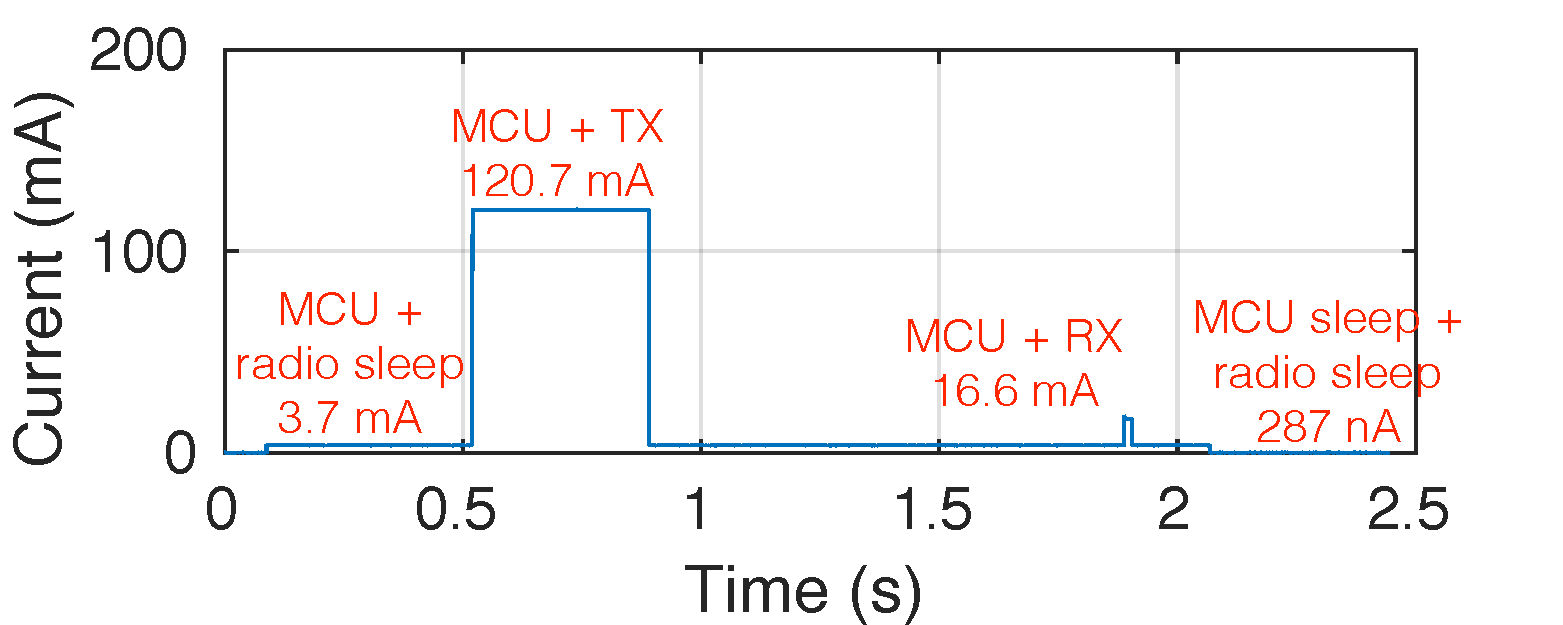
\includegraphics[width=0.36\textwidth]{figures/bug_power_trace_annotated}
\label{fig:power-trace}}\\
\hspace*{0.1in}
\subfloat[Estimated lifetime of a client device powered by two AA batteries sending 36 byte packets at various data rates based on the energy profile.]{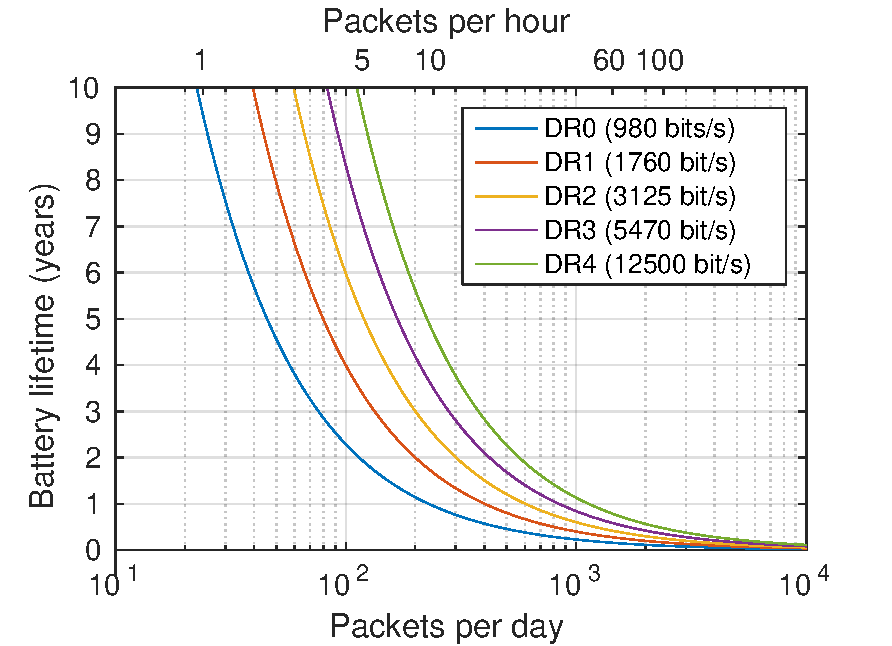
\includegraphics[width=0.36\textwidth]{figures/LoRaBug_AA_lifetime_semilog}
\label{fig:lifetime-estimates}}
\end{tabular}
\vspace*{-0.1in}
\caption{Power statistics}
\compactimg
\end{figure}

\section{Results}
\label{sec:eval}

%{\color{blue} }
%We implemented our system using 8 LPWAN boards as base stations distributed across a university campus.  We used a Semtech SX1276 LoRaWAN transmitter as the client device. We use Charm as the software platform at the backend to support backhaul. 

We evaluate \name\ both through
proof-of-concept experiments and large-scale trace-driven simulations. We
perform our experiments in various environments (indoors and outdoors) across the campus. 




\subsection{Role of Transmission Rates on Battery Life}
\label{sec:energy-savings}


% Most LP-WAN client devices are expected to be small, low-cost and low-maintenance battery-operated devices performing primarily some sensing functions. As these devices are expected to operate for many years, battery life is a major concern and is very difficult to optimize for. The amount of data to transmit is determined by the device and we do not attempt to alter it in this paper. Similarly, to maintain compatibility, we do not alter the MAC protocols or client device requirements specified in LoRaWAN.

We study the energy profile of a typical battery-operated LoRaWAN client, as in \figref{power-trace}. The device performs some local computation, sends a LoRa message, waits for an acknowledgement and then goes to low-power sleep mode. The radio transmission consumes the highest amount of energy ($= \text{area under the curve} \times \text{voltage}$) by a large margin. Thus, any optimization to battery life must focus on reducing the energy of transmissions.

Two parameters affect the energy consumed by transmissions: (1) transmit power and (2) transmit time. Using the currently available LoRa radio chipsets (Semtech SX1272 and SX1276), we've observed that the transmit power does not significantly change the power drawn from the battery during transmission. Any optimization will thus have to focus on reducing the transmit time. The transmit time is determined by the data rate and the amount of data to send. We do not control the amount of data generated by client devices and thus, improving the data rate would provide the largest improvements.

\begin{figure}[!h]
\centering
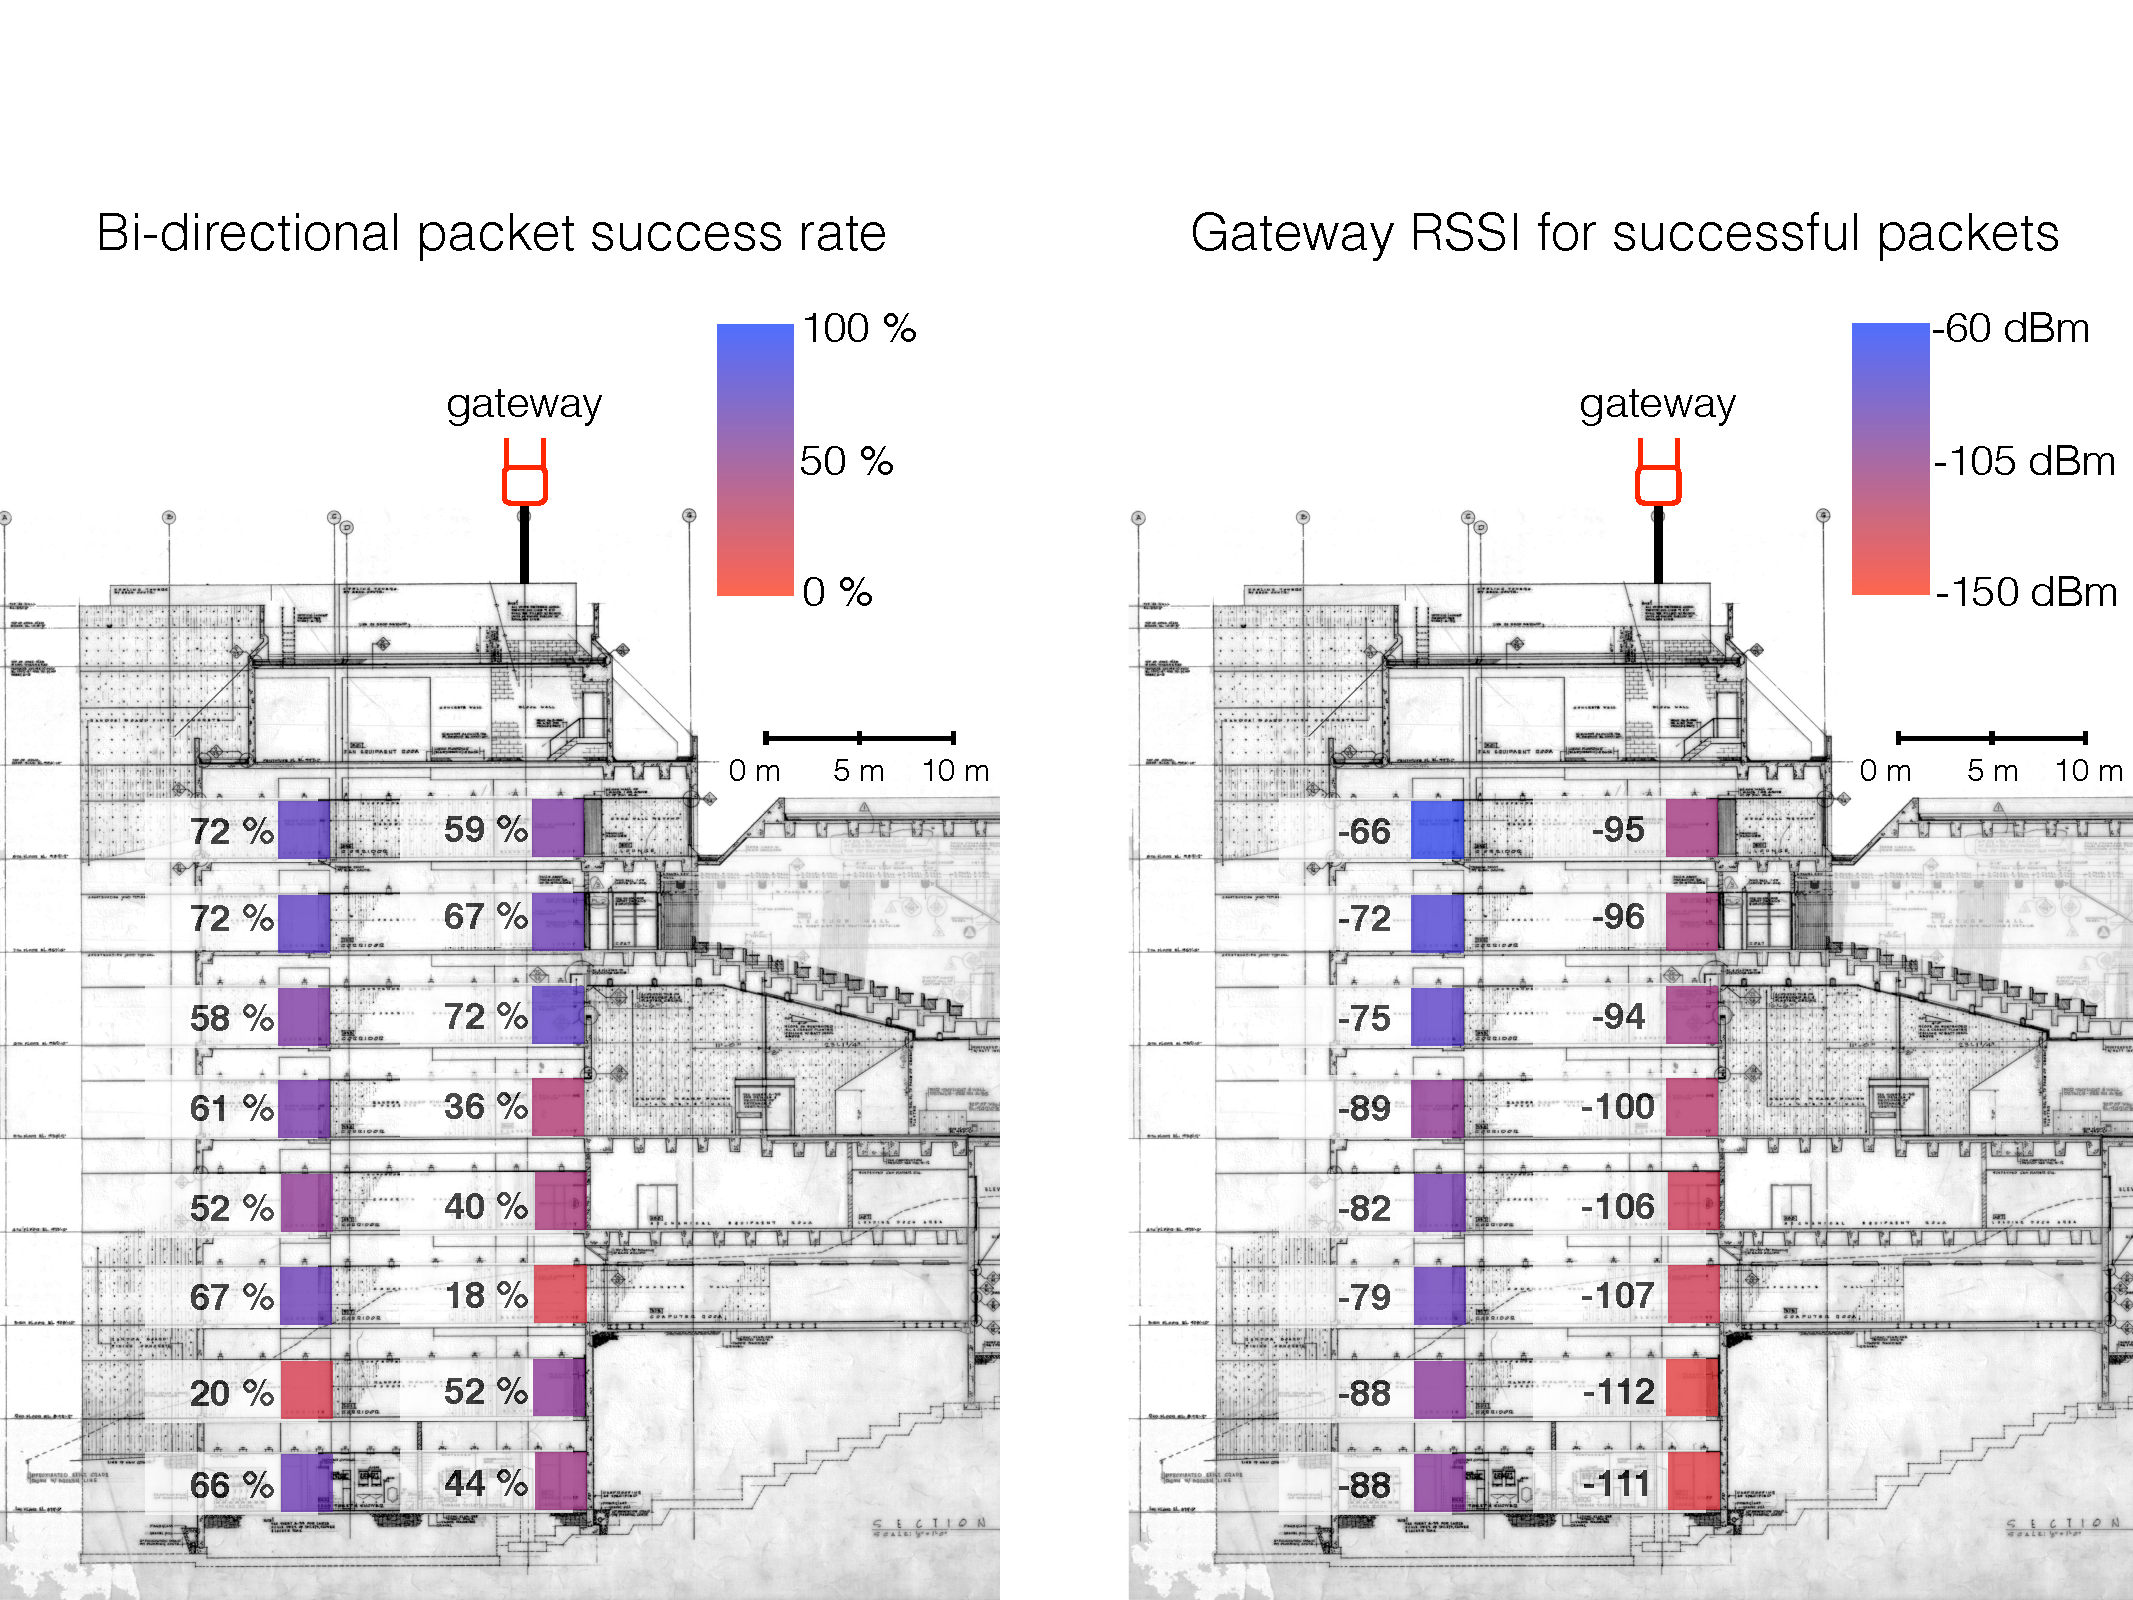
\includegraphics[width=0.35\textwidth]{figures/penetration_test_wean_cropped}
\caption{RF signal penetration experiments in a large poured-concrete building. (Left): the success rate for bi-directional packet exchange between end-node and gateway. (right): the RSSI at the gateway for successful transfers.}
\label{fig:penetration-test}
\compactimg
\end{figure}

\figref{lifetime-estimates} shows the estimated battery life of a client device if it were to communicate with different data rates. Wireless systems try to communicate at the highest data rate that does not cause too many errors. In the case of LoRa devices, switching to a slower data rate increases the spreading factor,  which have better sensitivity on the receiver. Thus, LoRa devices communicating at the highest spreading factors (and correspondingly using the lowest data rates) can communicate at much longer range and with higher reliability. The negative effect is a significant increase in their transmission time which severely affects battery life. This demonstrates that \name\ can significantly improve battery life should it allow clients to transmit at higher data rates. 

\begin{figure*}
\hfill
\begin{minipage}{.32\textwidth}
\centering
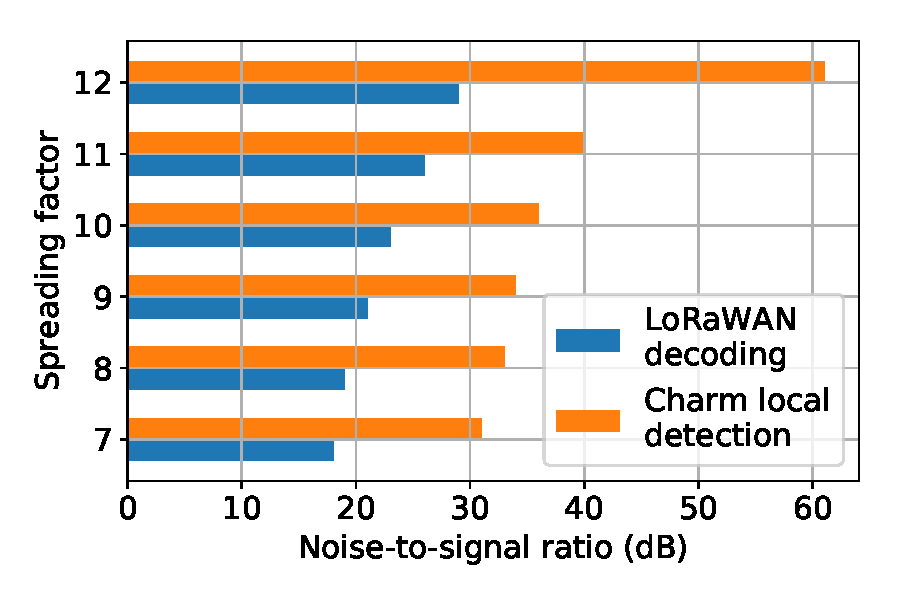
\includegraphics[width=0.95\textwidth]{figures/local_detection_limits}
\hspace*{-0.1in}
\caption{Local detection capacity at gateway for low SNRs}
\label{fig:local-detection}
\compactimg
\end{minipage}
\hfill
\begin{minipage}{.32\textwidth}
\centering
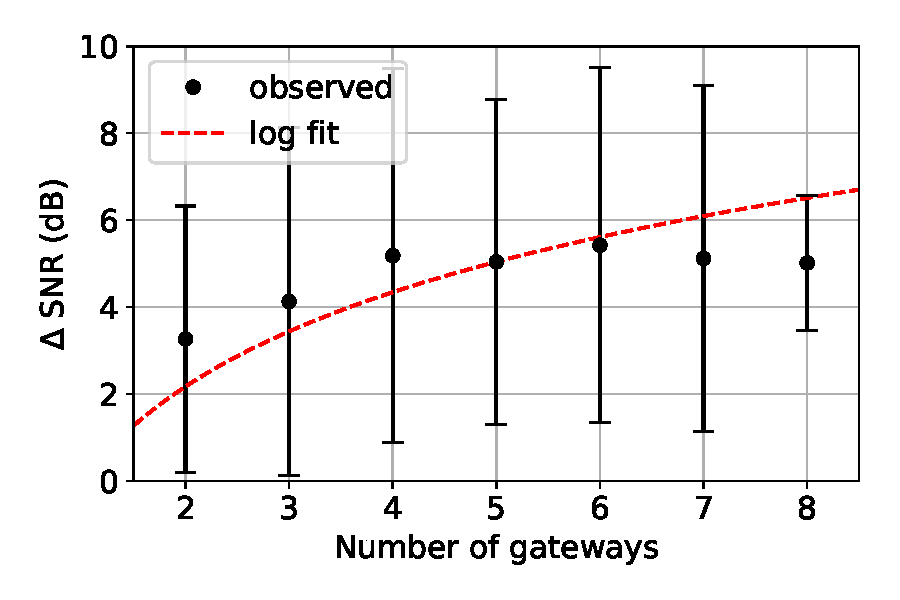
\includegraphics[width=0.95\textwidth]{figures/diversity_gain}
\hspace*{-0.1in}
\caption{Diversity gain with number of base stations}
\label{fig:diversity-gain}
\compactimg
\end{minipage}
\hfill
\begin{minipage}{.32\textwidth}
\centering
% Placeholder for adwait: Battery drain graph
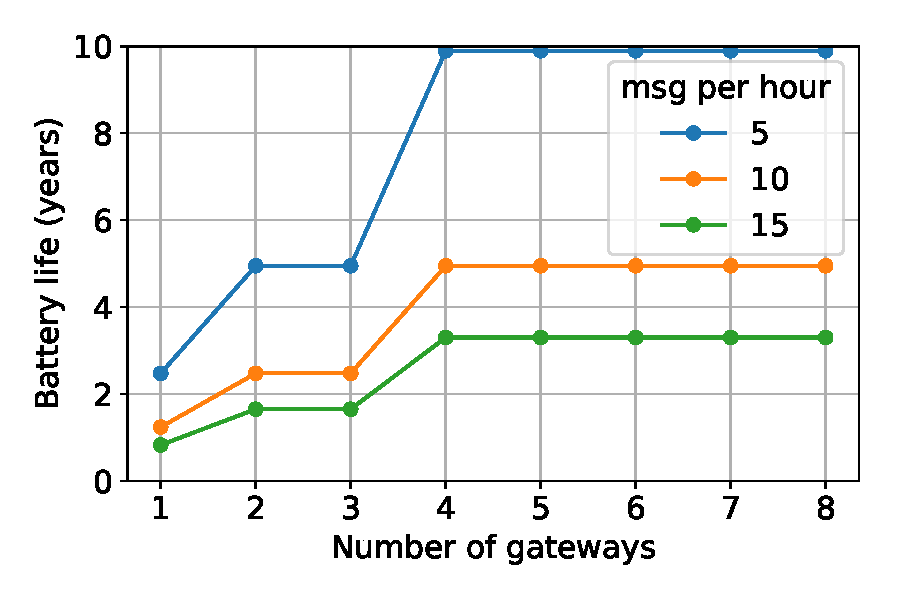
\includegraphics[width=0.95\textwidth]{figures/diversity_battery}
\hspace*{-0.1in}
\caption{Increase in battery life with number of base stations}
\label{fig:diversity-battery}
\compactimg
\end{minipage}
\end{figure*}

% Using Charm's joint decoding strategy, we enable devices previously forced to use low data rates due to distance or bad coverage, to communicate at higher data rates and lengthen their battery life. Devices which could previously communicate with at least one base stations using the highest data rate reliably, thus gain no benefit from Charm.



\name\ can not only increase coverage but also in urban scenarios with lots of obstructions and devices deep inside buildings. \figref{penetration-test} shows a penetration test experiment inside an on-campus poured-concrete building. Despite a gateway being placed on the roof of the building, we observe the received signal strength to vary as much as 46 dBm at various locations inside the building. A number of client devices, deep inside structure, would have been forced to use the the slowest data rate but can now benefit from Charm.

\subsection{Local detection algorithm}
\label{sec:local-detection-eval}



We performed trace-driven simulation to demonstrate the increase in detection capability of LoRa packets under noise. To perform this experiment, we collect data at different spreading factors at high SNRs. We then measure the signal power and progressively increase additive white Gaussian noise in the signal. At every dB of decrease in SNR, we test the state-of-the-art LoRaWAN decoding algorithm against Charm's local and enhanced detection algorithm, where the former uses the preamble alone and the latter uses both preamble and data in its optimization. 

The results in \figref{local-detection} show that \name's local detection algorithm far outperforms the LoRaWAN detection algorithm for detection of the packet. Further, \name's enhanced algorithm outperforms \name's local detection algorithm by up to 10 dB, as it uses data symbols in addition to the preamble, improving performance. This demonstrates the value of using data symbols to better optimize packet detection, particularly in noisy settings. Our results also reveal a 33\% increase in the negative SNR under which a packet can be detected, when compared to LoRaWAN -- a gain of between 16-30 dB. To put this in perspective, this is equivalent boost in SNR by coherent combining of between 40-1000 gateways. Said differently, \name\ can even detect packets that can only be decoded by coherently combining signals from at least 40 gateways that receive the same signal at a similar level of noise. 

% Swarun: Doesn't flow well
%Our results also reveal a 33\% increase in the negative SNR under which a packet can be detected, when compared to LoRaWAN. This increase of 33\% in power directly results in increase in coverage area of LoRa and improvement in battery-life for users already within coverage area. We also highlight how the enhanced algorithm is able to leverage the nature of the data to increase the quality of detection at extremely low SNRs. This shows that this algorithm can detect packets even under heavy noise from far or occluded locations which allows us to only send data to the cloud only when we detect the arrival of a packet. This lowers the bandwidth usage of the backbone network by reducing the amount of data that needs to be sent to the cloud. 
\subsection{Diversity gain}
\label{sec:diversity-gain-eval}

Next, we evaluate the  gain introduced by \name\ in signal-to-noise ratio (SNR) when coherently combining the multiple transmissions from geographically diverse receivers at a central server. We measure the mean and standard deviation in SNR improvement as a function of number of gateways across experiments.  

Our results reveal remarkable SNR improvements, which as expected improves steadily with an increasing number of gateways as depicted in Figure \ref{fig:diversity-gain}, for clients in different locations across multiple spreading factors. We note that the SNR gain improvement is logarithmic given that it is measured in dB (a log-scale). Across experiments, \name\ gave an average observable improvement of 1 dB with the addition of each new receiver. This improvement is valuable, given that every 3 dB of gain allows us to use the next spreading factor. Any increase in spreading factor halves the transmission air time and the resulting energy expenditure. \figref{diversity-battery} depicts the improvement in battery life of an indoor LoRaWAN client with an increasing number of gateways collaborating to decode its signal. We observe that the battery life for a device transmitting 5 messages per hour at SF11 improves from 2.5 years to 10 years (SF9) with 4 or more collaborating gateways


\subsection{Range Improvement for Indoor User-Deployed Gateways}

In typical urban settings, users will deploy large number of LoRa gateways. This increase in number of gateways reduces the range of a LoRa device and the bit-rate it can support even for hundreds of meters. We deploy \name\ in a highly congested urban building and can demonstrate that collaboration can improve the maximum range the LoRa device can support at any given data rate.


\begin{wraptable}{r}{4.5cm}
%\vspace*{-0.1in}
\centering \begin{tabular}{||c | c | c||} 
 \hline
  & \textbf{SF7} & \textbf{SF10} \\ [0.5ex] 
 \hline\hline
 \textbf{LoRa} & $<$60m & $<$60m  \\ 
 \hline
 \textbf{4 UDGs} & $<$60m & $<$100m  \\
 \hline
 \textbf{8 UDGs} & $<$200m & $<$200m \\
 \hline
\end{tabular}
\caption{Range in congested indoor urban settings}
\label{tab:range}
\vspace*{-0.1in}
\end{wraptable}

Our results are shown in Table~\ref{tab:range}. We compare the results of a single LoRa gateway with those of \name\ with 4 and 8 gateways collaborating, respectively. Note that the ranges we observe here are smaller than outdoor gateways, owing to attenuation inside buildings and limited transmission power. In this context, native LoRaWAN can at best reach 60~m of maximum range from any gateway. In contrast, \name\ consistently supports higher maximum range at each spreading factor. The results with \name\ using eight collaborating gateways show a marked improvement in range of 200 m, higher than 4 collaborating gateways at 100 m.



\begin{figure*}[htb]
\centering
\subfloat[Dense cells]{
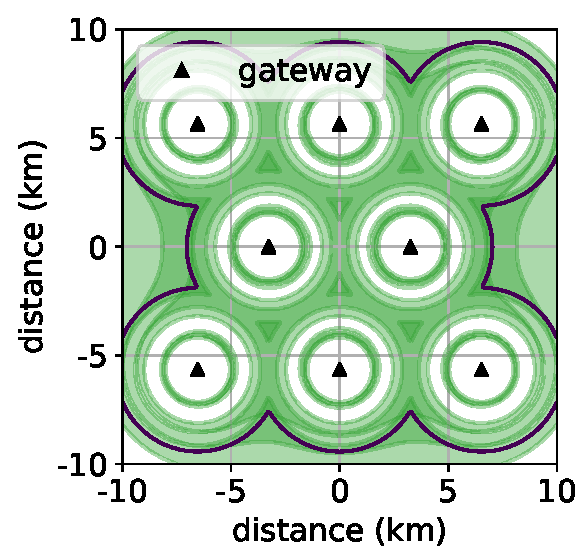
\includegraphics[width=0.3\textwidth]{figures/dense_cells_charm_improvement_cropped}
\label{fig:dense-improvement}
} \hfill
\subfloat[Sparse cells]{
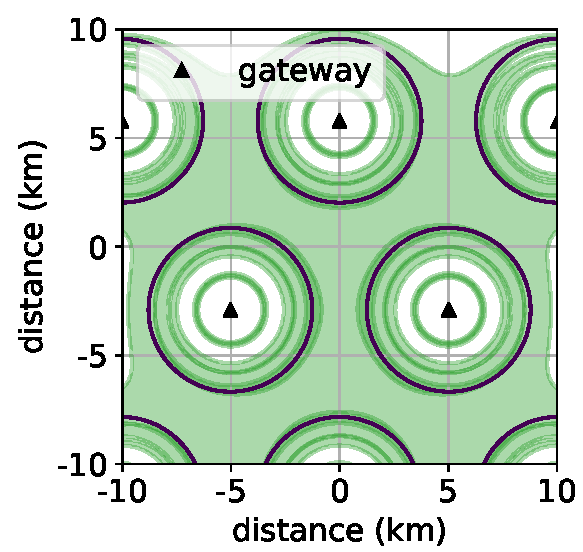
\includegraphics[width=0.3\textwidth]{figures/sparse_cells_charm_improvement_cropped}
\label{fig:sparse-improvement}
} \hfill
\subfloat[Random placement]{
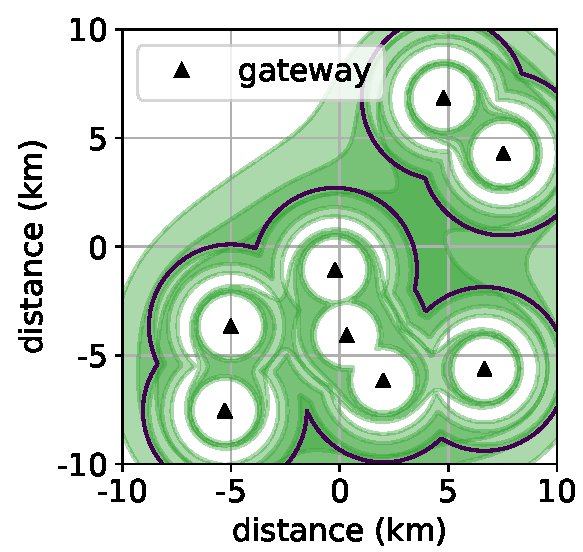
\includegraphics[width=0.3\textwidth]{figures/random_placement_charm_improvement_cropped}
\label{fig:random-improvement}
}
\compactimg
\caption{Improvement in coverage area and data rates due to Charm are shown by the green regions. The black lines show the coverage area with existing LoRaWAN. Darker regions denote greater gain in battery life.}
\label{fig:charm-improvement}
\compactimg
\end{figure*}


\subsection{Effect on coverage and client data rates}
\label{sec:coverage-data-rate-improvement}

This section uses trace-driven simulations to show the advantages of Charm in improving coverage area and client energy consumption in both planned and unplanned gateway deployments. We use the log-distance path loss model to estimate the signal power at any given receiver. The model is calibrated using 4850 points collected in a varied urban environment at varying data rates and spreading factors using a GPS-connected LoRa client device. Our log-distance parameters are $L_0  = 98.0729 dB$ for $d_0 = 40.0 m$, $\gamma = 2.1495$ and flat fading $\sigma^2 = 100.0724$. Sensitivity values for the gateway are taken from \cite{Bor2016} to determine the SNR threshold required to decode a transmission. Since this is an urban environment with many obstacles and reflectors, we observe a maximum range of 3.77 km using a transmit power of 15 dBm as opposed to the marketed range of 10 km with line-of-sight. We provide an optimistic estimate and ignore the effects of fading (assume $\sigma^2 = 0$) in the simulation, since we are interested in the trend of changes.

Assuming the same transmit power on the client of 15 dBm, \figref{charm-improvement} shows the region where Charm's local detection followed by joint decoding shows an improvement in either coverage, client data rates or both compared to independent decoding on gateways (as is currently done in LoRaWAN). Imagine the regions with no coverage having a data rate of DR``-1'' = 0 bps (the next lowest data rate is DR0 = 960 bps using SF = 12). Every shade of green represents a region where a client device can increase its data rate by one and correspondingly reduce its transmission time by approximately half. Darker green areas represent regions where devices can switch by more than one data rate. The areas enclosed within the black boundary are regions that could be covered by the existing LoRaWAN system (that decodes on each gateway independently). As can be seen in each of the sub-figures, Charm shows an improvement in the coverage area (green regions outside the existing coverage region), an increase in client data rates (green regions inside the existing coverage region) as well as both simultaneously (darker green areas outside the existing coverage area). Table~\ref{table:charm-improvements} shows the results of the simulations shown in \figref{charm-improvement}. Every increase in the data rate, doubles the battery life of a client device. Some regions in the simulation show up to 8 $\times$ energy savings.

\figref{dense-improvement} shows an ideal planned deployment where gateways are placed in a dense hexagonal grid 6.53 km apart from each other (corresponding to $2*3.77*\cos(\pi/6)$ km). Such an arrangement, popular in cellular deployments, provides optimal coverage with no gaps when using an independent decoding scheme. However, the points farthest from the gateways (e.g. on the centroid between three neighbouring gateways) have to use the slowest data rates (corresponding to SF12) and their battery life correspondingly suffers. If such a deployment were to be augmented with Charm, the region between the gateways can all communicate using SF9 or better. For the centroid points, this reduces the transmit time by approximately a factor of 8 and leads to huge energy savings. Additionally, we see the coverage area for joint decoding has expanded beyond the original coverage region. Some of the devices in the expanded coverage area can even communicate with higher data rates. An interesting phenomenon seen in each of the sub-figures are the thin concentric circles of improvement around each gateway. These are regions just outside the original boundaries covered by any given spreading factor that also gain a data rate increase due to joint decoding. However, this effect is not as prominent and the circles are small.

\figref{sparse-improvement} shows a sparse cellular arrangement with gateways 10.05 km apart from each other that can provide gap-free coverage. Charm thus enables decreasing the gateway density by a factor of 3.33 (proportional to square of inter-gateway distance $=(11.92/6.53)^2$) while providing the same level of coverage. Finally, we show in \figref{random-improvement} how Charm also improves the performance of an unplanned deployment of user-deployed gateways by improving coverage area as well as data rates for clients. Another interesting phenomenon to observe here is that Charm's joint decoding manages to fill in islands and orphaned regions. This is particularly relevant to urban regions where areas of bad coverage are formed in building basements and other indoor regions as seen in \figref{penetration-test}. 

\begin{table}[]
\centering
\caption{Summary of trace-driven simulation results shown in \figref{charm-improvement}}
\label{table:charm-improvements}
\begin{tabular}{l|l|l|l|}
\cline{2-4}
                                                       & \textbf{\begin{tabular}[c]{@{}l@{}}dense \\ cells\end{tabular}} & \textbf{\begin{tabular}[c]{@{}l@{}}sparse \\ cells\end{tabular}} & \textbf{\begin{tabular}[c]{@{}l@{}}random \\ placement\end{tabular}} \\ \hline
\multicolumn{1}{|l|}{\textbf{increase in coverage}}    & 46.60\%                                                         & 97.85\%                                                          & 74.59\%                                                              \\ \hline
\multicolumn{1}{|l|}{\textbf{data rate +1 (energy/2)}} & 35.33\%                                                         & 38.82\%                                                          & 33.70\%                                                              \\ \hline
\multicolumn{1}{|l|}{\textbf{data rate +2 (energy/4)}} & 22.30\%                                                         & 0\%                                                              & 25.82\%                                                              \\ \hline
\multicolumn{1}{|l|}{\textbf{data rate +3 (energy/8)}} & 2.26\%                                                          & 0\%                                                              & 3.48\%                                                               \\ \hline
\end{tabular}
\end{table}
